\documentclass[a4paper,12pt,landscape,twocolumn,gray]{article}

\usepackage{préambule}
\usetikzlibrary{positioning}
\usepackage{clipboard}

\setlength{\columnsep}{2cm}

\geometry{left=1cm,right=1cm}

\TitreDActivite{Activité : inégalité triangulaire}

\begin{document}

\Copy{Activité}{
	\maketitle

	\begin{greybox}[frametitle={Avant de commencer}]
		Le professeur va vous donner une feuille blanche.

		Sur cette feuille, découpez cinq bandes rectangulaires, de largeur \squared{5mm}, et de longueur respectives : \squared{3cm}, \squared{5cm}, \squared{7cm}, \squared{10cm} et \squared{12cm}.

		Marquez la longueur de chaque bande dessus. Vous pouvez aussi les colorier pour les différencier.

		\uline{Exemple :}

		\begin{center}
			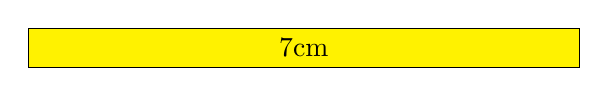
\begin{tikzpicture}
				\draw[fill=yellow] (0,0) rectangle node {7cm} (7,0.5);
			\end{tikzpicture}
		\end{center}
	\end{greybox}

	\begin{enumerate}
		\item Est-il possible de construire un triangle avec les bandes suivantes :
		      \begin{itemize}
			      \item 3cm, 5cm et 7cm ?
			      \item 5cm, 7cm et 10cm ?
			      \item 3cm, 5cm et 12cm ?
			      \item 12cm, 5cm et 7cm ?
			      \item 3cm, 5cm et 10cm ?
		      \end{itemize}
		\item \textbf{Sans réaliser de figure}, est-il possible de construire un triangles dont les côtés mesurent 21cm, 25cm et 42cm ?
		      \vspace{0.6em}

		      \dotfill
		\item Y-a-t'il une règle générale pour savoir si on peut construire un triangle ?
		      \vspace{1em}

		      \dotfill
	\end{enumerate}
}

\newpage

\Paste{Activité}

\end{document}